\documentclass[crop,tikz,10pt]{standalone}
\usepackage{tikz}
	\usetikzlibrary{shapes}
	\usetikzlibrary{automata}
	\usetikzlibrary{arrows}
	\usetikzlibrary{backgrounds}
	\usetikzlibrary{calc}
	\usetikzlibrary{positioning}
	\usetikzlibrary{patterns}
	\usetikzlibrary{decorations.pathmorphing}
	\usetikzlibrary{decorations.pathreplacing}

\usepackage[scaled]{helvet}
\renewcommand{\familydefault}{\sfdefault}

\usepackage{booktabs}
\usepackage{bm}
\usepackage{mhchem}
\usepackage{siunitx}
\usepackage{xcolor}
    \definecolor{TUMOrange}{RGB}{227, 114, 34}
    \definecolor{TUMBlueDark}{RGB}{0, 82, 147}

\input{../../../../resources/latex/_symbols.qmd}

\begin{document}

\newcommand{\n}[1]{\begin{tabular}{c}#1\end{tabular}}
\renewcommand{\vec}[1]{\boldsymbol{\mathbf{#1}}}

\pgfdeclarelayer{background}
\pgfdeclarelayer{foreground}

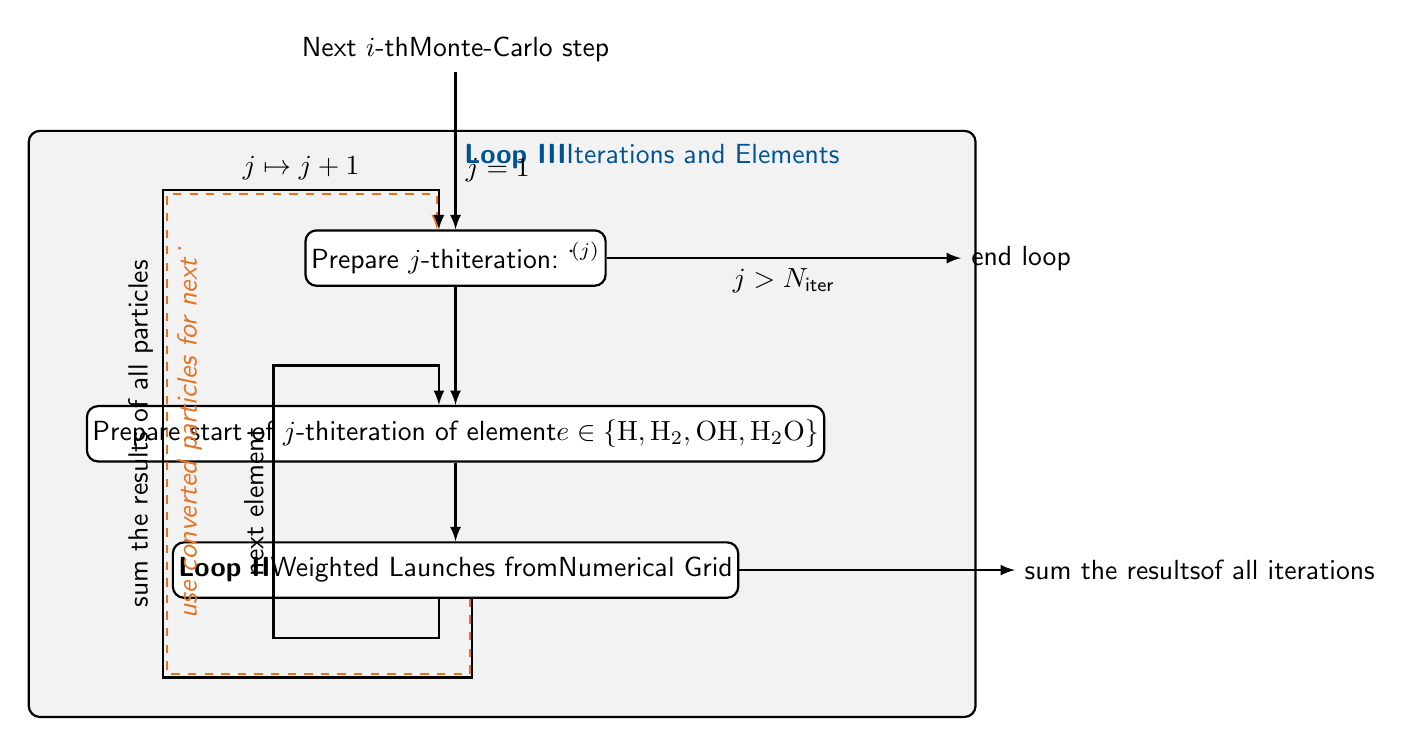
\begin{tikzpicture}[
    main/.style={draw, thick, rounded corners=4pt, inner sep=2pt, minimum size=20pt, minimum width=25pt, fill=white},
]

    %::. main nodes
    \node[main] (LOOPII) at (0,0) {\n{\textbf{Loop II} \\ Weighted Launches from \\ Numerical Grid}};
    \node[main, above = of LOOPII] (ELEMS) {\n{Prepare start of $j$-th \\ iteration of element \\ $e \in \left\{\ce{H}, \ce{H2}, \ce{OH}, \ce{H2O}\right\}$}};
    \node[main, above = 1.5 of ELEMS] (ITERATION) {\n{Prepare $j$-th \\ iteration: $\dot\source^{(j)}$}};

    %::. main connections
    \draw[-latex, thick] (ELEMS.270) -- (LOOPII.90);
    \draw[-latex, thick] (ITERATION.270) -- (ELEMS.90);

    \draw[-latex, thick] (LOOPII.240) |- +(-1,-0.5) -| node[near end, left, above, rotate=90] {next element} ($(ELEMS.120) + (-2.1, 0.5)$) -| (ELEMS.120);

    \draw[-latex, thick, TUMOrange, dashed] (LOOPII.297) |- +(-1,-0.95) -| node[near end, left, below, rotate=90] {\emph{use converted particles for next $\dot\source$}} ($(ITERATION.123) + (-3.425, 0.45)$) -| (ITERATION.123);
    \draw[-latex, thick] (LOOPII.300) |- +(-1,-1) -| node[near end, left, above, rotate=90] {sum the results of all particles} ($(ITERATION.120) + (-3.5, 0.5)$) -| (ITERATION.120) node[near start, above] {$j\mapsto j+1$};

    %::. exit node
    \node[right = 3.5 of LOOPII] (SUM) {\n{sum the results \\ of all iterations}};

    %:: exit node connection
    \draw[-latex, thick] (LOOPII.0) -- (SUM.180);
    \draw[-latex, thick] (ITERATION.0) -- +(4.5,0) node[midway, below]{$j > N_\text{iter}$} node[at end, right] {end loop};

    %::. input connection
    \draw[latex-, thick] (ITERATION.90) -- +(0,2) node[midway, right, yshift=-7px]{$j=1$} node[at end, above] {\n{Next $i$-th \\ Monte-Carlo step}};


    %::. background loop node
    \begin{pgfonlayer}{background}
        \draw[thick, fill=white!95!black, rounded corners=4pt] ($(ITERATION.north west) + (-3.5, 1.25)$) rectangle ($(LOOPII.south east) + (3, -1.5)$);
        \node[anchor=north east, text=TUMBlueDark] at ($(ITERATION.90) + (5.0, 1.2)$) {\n{\textbf{Loop III} \\ Iterations and Elements}};
    \end{pgfonlayer}
\end{tikzpicture}

\end{document}